\begin{figure}[p]
  \centering
  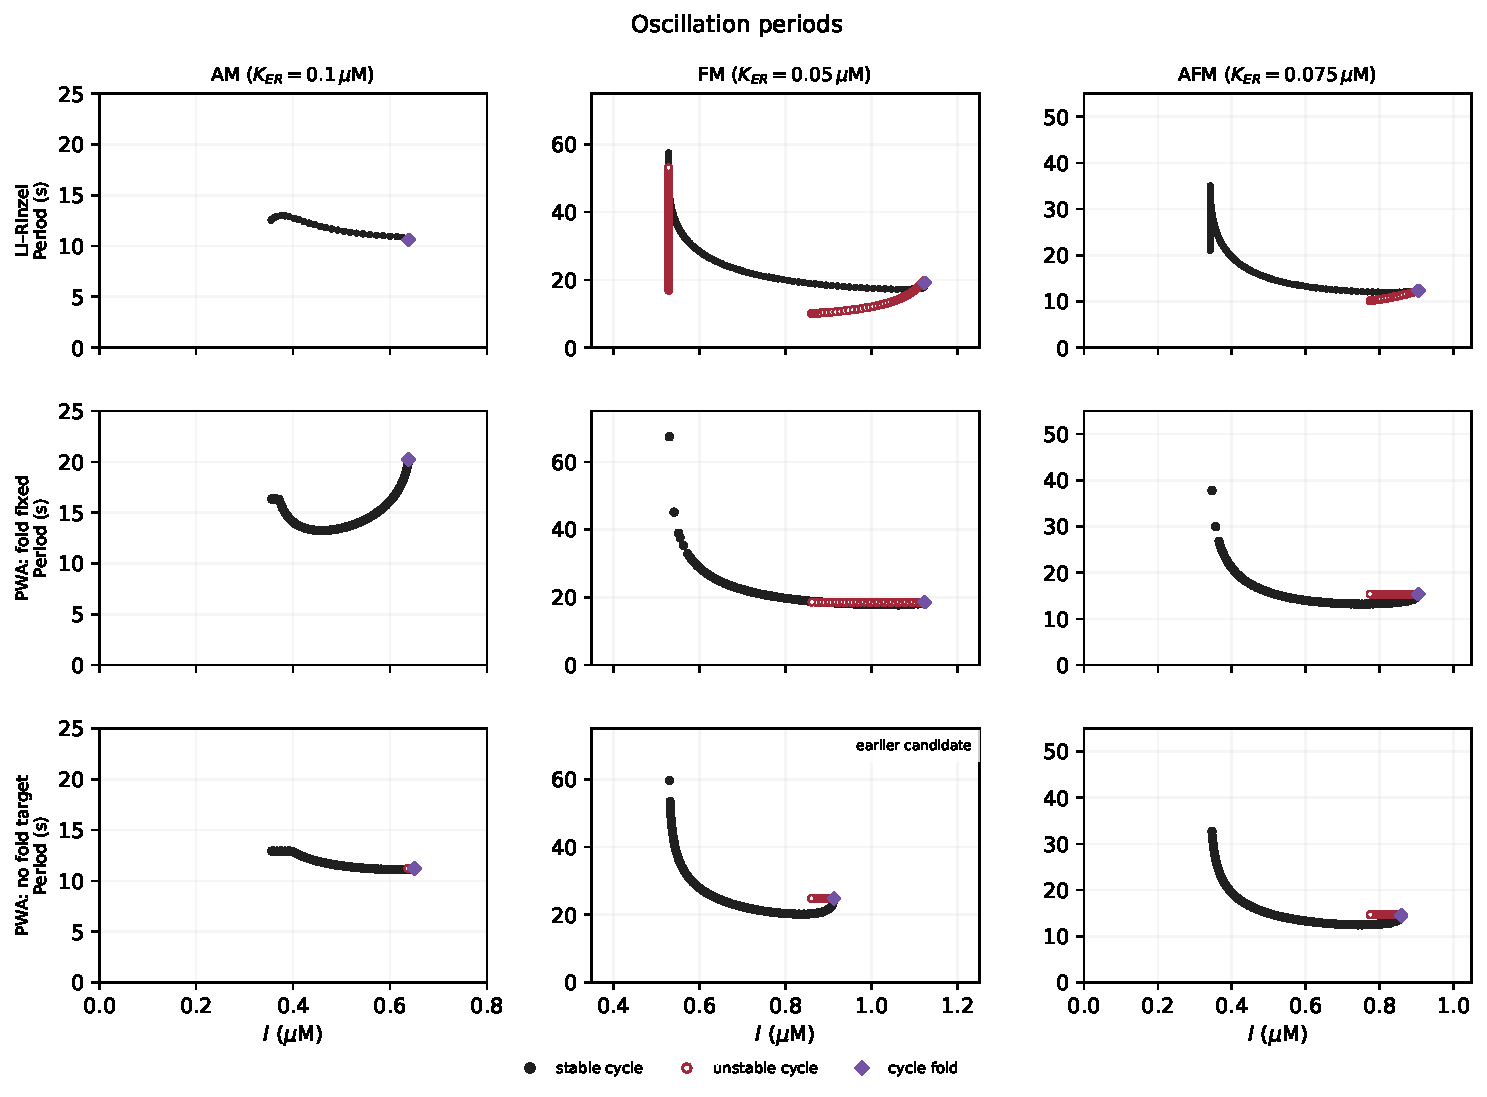
\includegraphics[width=\linewidth]{figures/figure5_period_comparison.pdf}
  \caption{Periods of Li--Rinzel and mixed-coordinate two-threshold PWA models for AM, FM, and AFM parameter regimes. Columns indicate the regimes; rows show the reference, PWA fitted with the upper cycle fold constrained, and PWA fitted without a fold constraint. Filled black and open red circles denote stable and unstable periodic orbits, respectively; diamonds denote computed cycle folds. In the lower row the folds are numerical candidates found after fitting, not imposed targets. Li--Rinzel data use collocation continuation with independent finite-time checks. PWA data use finite forward trajectory scans, boundary matching, pseudo-arclength continuation and independent forward or backward integration checks. Missing branches do not prove absence. The FM PWA without fold constraint is an earlier archive candidate; the final frozen FM candidate was unavailable locally.}
  \label{fig:period-comparison}
\end{figure}
